\documentclass[12pt,a4paper]{article}

% --- Encoding / fonts / language ---
\usepackage[T1]{fontenc}
\usepackage[utf8]{inputenc}
\DeclareUnicodeCharacter{00A0}{~}
\usepackage{lmodern}
\usepackage[ngerman]{babel}
\usepackage{microtype}

% --- Graphics / links / color ---
\usepackage{graphicx}
\usepackage{hyperref}
\usepackage{xurl}
\usepackage{xcolor}

\graphicspath{{diagrams/}}
\usepackage{float}

% --- Tables ---
\usepackage{array}
\usepackage{ragged2e}
\usepackage{tabularx}
\usepackage{longtable}
\usepackage{ltablex}
\keepXColumns

% --- Code / listings ---
\usepackage{listings}
\usepackage{listingsutf8}
\lstset{inputencoding=utf8/latin1}

% --- Page geometry ---
\usepackage{geometry}
\geometry{a4paper, top=20mm, left=20mm, right=20mm, bottom=25mm}

% --- Headers / footers ---
\usepackage{fancyhdr}
\setlength{\headheight}{15pt}
\pagestyle{fancy}
\lhead{Luca Güttinger}
\rhead{\today}
\rfoot{Seite \thepage}
\cfoot{}
\lfoot{\footnotesize\mbox{\url{https://github.com/Notenverwaltung-ch/Notenverwaltung}}}

% --- Listings config ---
\lstset{
    inputencoding=utf8,
    language=SQL,
    basicstyle=\small\ttfamily,
    breaklines=true,
    breakatwhitespace=true,
    columns=fullflexible,
    keepspaces=true,
    showstringspaces=false,
    tabsize=2,
    postbreak=\mbox{\textcolor{red}{$\hookrightarrow$}\space}
}

% --- Helpers ---
\newcommand{\code}[1]{\texttt{\detokenize{#1}}}

% --- Column types for tables ---
\newcolumntype{L}[1]{>{\raggedright\arraybackslash}p{#1}}
\newcolumntype{C}[1]{>{\centering\arraybackslash}p{#1}}
\newcolumntype{R}[1]{>{\raggedleft\arraybackslash}p{#1}}
\newcolumntype{Y}{>{\raggedright\arraybackslash}X}

\setlength{\parindent}{0pt}
\setlength{\parskip}{6pt}

\setcounter{tocdepth}{4}
\setcounter{secnumdepth}{4}

\begin{document}
    \hypersetup{pageanchor=false}
% ---------------- Titelseite ----------------
    \begin{titlepage}
        \centering
        {\huge\bfseries Notenverwaltungssystem \par}
        \vspace{2cm}
        {\Large Luca Güttinger \par}
        \vspace{0.5cm}
        {\Large Dipl. Informatiker Applikationsentwicklung \par}
        \vspace{0.5cm}
        {\Large TEKO Zürich \par}
        \vspace{0.5cm}
        {\Large Datenbanken / Big Data / Data Cubes \par}
        {\Large Dozent: Milad Fakiry \par}
        \vspace{0.5cm}
        {\Large Abgabedatum: 07.09.2025 \par}
        \vfill
    \end{titlepage}
    \clearpage
    \hypersetup{pageanchor=true}
    \pagenumbering{arabic}

% ---------------- Inhaltsverzeichnis ----------------
    \tableofcontents
    \newpage

% ---------------- Einleitung ----------------
    \section{Einleitung}
    In diesem Projekt wurde ein Notenverwaltungssystem für die Website Notenverwaltung.ch entwickelt.
    Das Szenario sieht vor, dass Schülerinnen und Schüler ihre eigenen Noten jederzeit einsehen und verwalten können, auch unabhängig von Lehrpersonen.
    Zusätzlich können optionale Verwaltungsfunktionen für Fächer, Klassen, Tests und Semester genutzt werden,
    sofern diese von einer Schule oder Lehrperson bereitgestellt werden.
    Die Anwendung besteht aus einer PostgreSQL-Datenbank und einem Spring Boot Service, welcher über eine REST-API zugänglich ist.
    Die Endpunkte sind durch JWT-Token abgesichert und es existieren verschiedene Rollen (z. B. \code{STUDENT}, \code{TEACHER}, \code{ADMIN}).

    \subsection{Ziel der Arbeit}
    Ziel der Arbeit ist es, ein Backend für Notenverwaltung.ch zu konzipieren und umzusetzen,
    das insbesondere die eigenständige Notenverwaltung durch Schülerinnen und Schüler ermöglicht, unabhängig von Lehrpersonen. Im Fokus stehen:
    \begin{itemize}
        \item eine saubere relationale Datenbankstruktur,
        \item eine klar dokumentierte REST-API (Spring Boot) für das Erfassen, Bearbeiten und Auswerten persönlicher Leistungen,
        \item Authentifizierung und Autorisierung mittels JWT mit Rollen (z. B. \code{STUDENT}, \code{TEACHER}, \code{ADMIN}),
        \item optionale Anbindung schulischer Strukturen (Fächer, Klassen, Tests, Semester), sofern verfügbar.
    \end{itemize}

    \subsection{Abgrenzung}
    Teil der Arbeit ist die Datenmodellierung, SQL-Implementierung, beispielhafte Abfragen und ein Testprotokoll.
    Ebenso wird die Absicherung der Schnittstellen (JWT) und eine rollenbasierte Zugriffskontrolle
    (z. B. \code{STUDENT}, \code{TEACHER}, \code{ADMIN}) umgesetzt. Nicht Teil der Arbeit ist eine vollständige,
    produktiv eingesetzte Frontend-Weboberfläche oder die Integration in bestehende Schulinfrastrukturen; der Fokus
    liegt auf der Backend-Funktionalität für Notenverwaltung.ch. Ein eigenständiges Frontend (z. B. mit Angular) ist
    im Rahmen dieser Arbeit nicht vorgesehen oder höchstens als sehr rudimentärer Prototyp zur Veranschaulichung der API gedacht.

% ---------------- Anforderungsanalyse ----------------
    \section{Anforderungsanalyse}
    Im Mittelpunkt steht, dass Schülerinnen und Schüler sich registrieren bzw. anmelden, ihre persönlichen Noten sicher einsehen,
    erfassen und bei Bedarf bearbeiten sowie Auswertungen über ihre Leistungen vornehmen können.
    Lehrpersonen und Admins erhalten, soweit vorgesehen, erweiterte Funktionen zur optionalen Verwaltung von Fächern, Klassen, Tests und Semestern.
    Sicherheitsanforderungen (JWT-basierte Authentifizierung und rollenbasierte Autorisierung), Datenkonsistenz, Nachvollziehbarkeit von Änderungen
    und der Schutz personenbezogener Daten (Datensparsamkeit, Zugriff nur für Berechtigte) sind zentrale nicht‑funktionale Anforderungen.

    \subsubsection{Funktionale Anforderungen}
    \begin{itemize}
        \item Registrierung und Anmeldung von Nutzerinnen und Nutzern (STUDENT, optional TEACHER/ADMIN).
        \item Selbstständige Verwaltung persönlicher Noten durch STUDENTs: Anlegen, Bearbeiten, Löschen von Tests/Noten im eigenen Bereich.
        \item Einsicht in Notenverläufe, Berechnung von Durchschnittswerten und einfachen Auswertungen pro Fach/Semester.
        \item Optionale Verwaltungsfunktionen für TEACHER/ADMIN: Fächer, Klassen, Tests und Semester anlegen und zuordnen.
        \item Rollenbasierter Zugriff auf REST-API-Endpunkte mit klar definierten Berechtigungen.
        \item Export einfacher Auswertungen (z. B. CSV/JSON) über die API (optional).
        \item Änderungsnachvollziehbarkeit für sensible Aktionen (z. B. wer hat welche Note wann geändert), soweit vorgesehen.
        \item Fehlermeldungen und Validierungen (z. B. Pflichtfelder, Wertebereiche, Dublettenprüfung bei eindeutigen Attributen).
    \end{itemize}

    \subsubsection{Nicht-funktionale Anforderungen}
    \begin{itemize}
        \item Sicherheit: JWT-basierte Authentifizierung, rollenbasierte Autorisierung, sichere Passwortspeicherung (Hashing), minimale Datenspeicherung.
        \item Datenqualität: Konsistenz durch Constraints/Referentielle Integrität, Transaktionssicherheit und Validierungen im Service.
        \item Performance und Skalierbarkeit: REST-API mit angemessenen Antwortzeiten unter typischer Last; effiziente Abfragen/Indizes.
        \item Verfügbarkeit und Betrieb: Containerisierbar (Docker), reproduzierbare lokale Entwicklung (docker-compose), einfache Deployment-Pfade.
        \item Nachvollziehbarkeit/Logging: Sinnvolle Server-Logs für Diagnose und Audit-Zwecke ohne sensible Daten im Klartext.
        \item Benutzbarkeit der API: Konsistente Endpunkte, klare Fehlercodes/-nachrichten und grundlegende Dokumentation (z. B. OpenAPI/HTTP-Beispiele).
        \item Wartbarkeit: Saubere Schichtung (Controller/Service/Repository), klare Domänenbegriffe, Tests für Kernfunktionen.
    \end{itemize}

    Die folgenden Entitäten und Beziehungen bilden diese Anforderungen im Datenmodell ab.

    Die realen Entitäten im Szenario sind:

    \begin{itemize}
        \item \textbf{Semester}: Zeitraum mit Start- und Enddatum, in dem Fächer angeboten werden.
        \item \textbf{Fach (Subject)}: Lehrfach, das in Semestern angeboten wird.
        \item \textbf{Klasse}: Gruppe von Studierenden, die ein Semesterfach besuchen.
        \item \textbf{Test}: Prüfung oder Klausur, die einer Klasse zugeordnet ist.
        \item \textbf{Note (Grade)}: Bewertung eines Tests für einen Studierenden.
        \item \textbf{Benutzer (User)}: Person mit Login-Daten für das System. Kann ein Schüler, eine Lehrperson oder ein Admin sein.
        \item \textbf{Rolle (UserRole)}: Zugriffsrechte für Benutzer (z. B. \code{STUDENT}, \code{TEACHER}, \code{ADMIN}).
    \end{itemize}

    Die Beziehungen:
    \begin{itemize}
        \item Ein \textbf{Semester} hat mehrere \textbf{Semesterfächer}.
        \item Ein \textbf{Fach} kann in mehreren \textbf{Semestern} vorkommen.
        \item Ein \textbf{Semesterfach} kann mehrere \textbf{Klassen} haben.
        \item Eine \textbf{Klasse} hat mehrere \textbf{Tests}.
        \item Ein \textbf{Test} hat mehrere \textbf{Noten}.
        \item Ein \textbf{Student} kann mehrere \textbf{Noten} haben.
        \item Ein \textbf{Benutzer} kann mehrere Rollen haben.
    \end{itemize}

% ---------------- Datenmodell ----------------
    \section{Datenmodell}

    \subsection{ER-Diagramm}
    Das folgende ER-Diagramm stellt die Entitäten, deren Attribute und die Beziehungen mit Kardinalitäten dar:

    \begin{figure}[H]
        \centering
        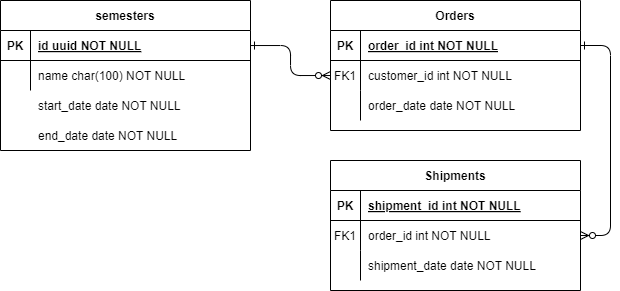
\includegraphics[scale=0.65]{diagrams/nv-erd}
        \caption{ER-Diagramm des Notenverwaltungssystems}
        \label{fig:erd}
    \end{figure}

    \subsection{Tabellenbeschreibung}
    Im Folgenden werden die Tabellen detailliert beschrieben. Für jede Entität gibt es eine separate Tabelle mit Attributen, Datentypen, Pflichten und Schlüsseln.

    \subsubsection{semesters}
    \begin{longtable}{|L{4cm}|L{3cm}|L{3cm}|L{4cm}|}
        \hline
        \textbf{Attribut} & \textbf{Datentyp} & \textbf{Pflicht} & \textbf{Bemerkung} \\ \hline
        id & uuid & ja & Primärschlüssel \\ \hline
        name & varchar(100) & ja & z. B. HS2025 \\ \hline
        start\_date & date & ja &  \\ \hline
        end\_date & date & ja &  \\ \hline
    \end{longtable}
    \textbf{Schlüssel / Constraints:} PK: id

    \subsubsection{subjects}
    \begin{longtable}{|L{4cm}|L{3cm}|L{3cm}|L{4cm}|}
        \hline
        \textbf{Attribut} & \textbf{Datentyp} & \textbf{Pflicht} & \textbf{Bemerkung} \\ \hline
        id & uuid & ja & Primärschlüssel \\ \hline
        name & varchar(150) & ja & Eindeutig (Unique) empfohlen \\ \hline
    \end{longtable}
    \textbf{Schlüssel / Constraints:} PK: id

    \subsubsection{semester\_subjects}
    \begin{longtable}{|L{4cm}|L{3cm}|L{3cm}|L{4cm}|}
        \hline
        \textbf{Attribut} & \textbf{Datentyp} & \textbf{Pflicht} & \textbf{Bemerkung} \\ \hline
        id & uuid & ja & Primärschlüssel \\ \hline
        semester\_id & uuid & ja & FK $\rightarrow$ semesters(id) \\ \hline
        subject\_id & uuid & ja & FK $\rightarrow$ subjects(id) \\ \hline
    \end{longtable}
    \textbf{Schlüssel / Constraints:} PK: id; Unique(semester\_id, subject\_id) empfohlen

    \subsubsection{classes}
    \begin{longtable}{|L{4cm}|L{3cm}|L{3cm}|L{4cm}|}
        \hline
        \textbf{Attribut} & \textbf{Datentyp} & \textbf{Pflicht} & \textbf{Bemerkung} \\ \hline
        id & uuid & ja & Primärschlüssel \\ \hline
        semester\_subject\_id & uuid & ja & FK $\rightarrow$ semester\_subjects(id) \\ \hline
        name & varchar(100) & nein & optionale Klassenbezeichnung \\ \hline
    \end{longtable}
    \textbf{Schlüssel / Constraints:} PK: id; FK: semester\_subject\_id

    \subsubsection{tests}
    \begin{longtable}{|L{4cm}|L{3cm}|L{3cm}|L{4cm}|}
        \hline
        \textbf{Attribut} & \textbf{Datentyp} & \textbf{Pflicht} & \textbf{Bemerkung} \\ \hline
        id & uuid & ja & Primärschlüssel \\ \hline
        name & varchar(150) & ja &  \\ \hline
        class\_id & uuid & ja & FK $\rightarrow$ classes(id) \\ \hline
        semester\_subject\_id & uuid & ja & FK $\rightarrow$ semester\_subjects(id) \\ \hline
        max\_points & numeric(10,2) & nein &  \\ \hline
        date & date & nein &  \\ \hline
    \end{longtable}
    \textbf{Schlüssel / Constraints:} PK: id; FK: class\_id; FK: semester\_subject\_id

    \subsubsection{grades}
    \begin{longtable}{|L{4cm}|L{3cm}|L{3cm}|L{4cm}|}
        \hline
        \textbf{Attribut} & \textbf{Datentyp} & \textbf{Pflicht} & \textbf{Bemerkung} \\ \hline
        id & uuid & ja & Primärschlüssel \\ \hline
        value & numeric(4,2) & ja & Notenwert (z. B. 1.0-6.0) \\ \hline
        weight & numeric(4,2) & nein & Gewichtung in Prozent \\ \hline
        student\_id & uuid & ja & FK $\rightarrow$ students(id) \\ \hline
        test\_id & uuid & ja & FK $\rightarrow$ tests(id) \\ \hline
        comment & varchar(255) & nein & Freitext \\ \hline
    \end{longtable}
    \textbf{Schlüssel / Constraints:} PK: id; FK: student\_id; FK: test\_id; Unique(student\_id, test\_id) empfohlen

    \subsubsection{users}
    \begin{longtable}{|L{4cm}|L{3cm}|L{3cm}|L{4cm}|}
        \hline
        \textbf{Attribut} & \textbf{Datentyp} & \textbf{Pflicht} & \textbf{Bemerkung} \\ \hline
        id & uuid & ja & Primärschlüssel \\ \hline
        username & varchar(100) & ja & Eindeutig (Unique) \\ \hline
        password & varchar(255) & ja & Hash (BCrypt) \\ \hline
        email & varchar(255) & ja & Eindeutig (Unique) empfohlen \\ \hline
        first\_name & varchar(100) & nein &  \\ \hline
        last\_name & varchar(100) & nein &  \\ \hline
        student\_number & varchar(50) & nein & Referenz auf Student möglich \\ \hline
        active & boolean & ja & Default: true \\ \hline
        created\_at & timestamp & ja &  \\ \hline
        updated\_at & timestamp & nein &  \\ \hline
    \end{longtable}
    \textbf{Schlüssel / Constraints:} PK: id

    \subsubsection{user\_roles}
    \begin{longtable}{|L{4cm}|L{3cm}|L{3cm}|L{4cm}|}
        \hline
        \textbf{Attribut} & \textbf{Datentyp} & \textbf{Pflicht} & \textbf{Bemerkung} \\ \hline
        user\_id & uuid & ja & FK $\rightarrow$ users(id) \\ \hline
        role & varchar(50) & ja & z. B. ADMIN, USER \\ \hline
    \end{longtable}
    \textbf{Schlüssel / Constraints:} PK: (user\_id, role); FK: user\_id
    \newpage

% ---------------- SQL-Implementierung ----------------
    \section{SQL-Implementierung}

    \subsection{CREATE TABLE Befehle}
    \begin{lstlisting}
CREATE TABLE public.students (
  id uuid PRIMARY KEY,
  first_name varchar(100) NOT NULL,
  last_name varchar(100) NOT NULL,
  email varchar(255) NOT NULL,
  date_of_birth date,
  student_number varchar(50) NOT NULL,
  active boolean DEFAULT true NOT NULL,
  created_at timestamp NOT NULL,
  updated_at timestamp
);
-- Weitere Tabellen siehe Anhang
    \end{lstlisting}

    \subsection{Beispielhafte INSERT-Befehle}
    \begin{lstlisting}
INSERT INTO students (
  id,
  first_name,
  last_name,
  email,
  student_number,
  created_at,
  updated_at
) VALUES (
  gen_random_uuid(),
  'Max',
  'Mustermann',
  'max@uni.de',
  'S12345',
  now(),
  now()
);

INSERT INTO subjects (
  id,
  name
) VALUES (
  gen_random_uuid(),
  'Mathematik'
);
    \end{lstlisting}

% ---------------- Beispielabfragen ----------------
    \section{Beispielabfragen / UI}

    \subsection{SQL-Abfragen}
    \begin{lstlisting}[language=SQL]
-- Alle Noten eines Studenten
SELECT s.first_name, s.last_name, g.value, t.name
FROM grades g
JOIN students s ON g.student_id = s.id
JOIN tests t ON g.test_id = t.id
WHERE s.student_number = 'S12345';
    \end{lstlisting}

    \textbf{Beispielausgabe:}
    \begin{verbatim}
Max Mustermann | 5.50 | Mathematik Test 1
Max Mustermann | 4.75 | Informatik Test 1
    \end{verbatim}

    \textbf{TODO: Screenshot aus DB-Client einfügen}
    \newpage

% ---------------- Testprotokoll ----------------
    \section{Testprotokoll}

    \subsection{Beschreibung}
    Die Tests wurden sowohl mit manuellen SQL-Abfragen als auch über die REST-API (gesichert durch JWT) durchgeführt.

    \subsection{Testfälle}\label{sec:testfaelle}

    \subsubsection{T1 - Student anlegen (gültige Daten)}
    \begin{small}
        \begin{tabularx}{\textwidth}{|L{3.2cm}|Y|}
            \hline
            \textbf{Feld} & \textbf{Wert} \\ \hline
            ID & T1 \\ \hline
            Erwartet & Student wird gespeichert \\ \hline
            Status & Pass \\ \hline
            Datum/Tester & 2025-09-04 / Luca G. \\ \hline
            ENV & DEV (Docker, Postgres 16, SB 3.3) \\ \hline
            Pre-Conditions & Admin-Token vorhanden; keine vorhandenen Studenten mit \code{student_number=S12345} \\ \hline
            Endpoint/Schritte & \code{POST /api/students} mit Body \code{\{first_name, last_name, email, student_number\}} \\ \hline
            Response (gekürzt) & \code{201 Created}; JSON mit \code{id, first_name, last_name, email, student_number} \\ \hline
            Post-Conditions & Student existiert in Tabelle \code{students}; Auditfelder gesetzt \\ \hline
            Referenz & REQ-STU-001 \\ \hline
        \end{tabularx}
    \end{small}

    \subsubsection{T2 - Student anlegen (fehlende Pflichtfelder)}
    \begin{small}
        \begin{tabularx}{\textwidth}{|L{3.2cm}|Y|}
            \hline
            \textbf{Feld} & \textbf{Wert} \\ \hline
            ID & T2 \\ \hline
            Erwartet & HTTP 400 Validierung \\ \hline
            Status & Pass \\ \hline
            Datum/Tester & 2025-09-04 / Luca G. \\ \hline
            ENV & DEV \\ \hline
            Pre-Conditions & Request ohne Pflichtfelder \\ \hline
            Endpoint/Schritte & \code{POST /api/students} (ungültiger Body) \\ \hline
            Response (gekürzt) & \code{400 Bad Request} mit Validierungsfehlern \\ \hline
            Post-Conditions & Kein Datensatz angelegt \\ \hline
            Referenz & REQ-STU-002 \\ \hline
        \end{tabularx}
    \end{small}

    \subsubsection{T3 - Semester hinzufügen}
    \begin{small}
        \begin{tabularx}{\textwidth}{|L{3.2cm}|Y|}
            \hline
            \textbf{Feld} & \textbf{Wert} \\ \hline
            ID & T3 \\ \hline
            Erwartet & In Liste sichtbar \\ \hline
            Status & Pass \\ \hline
            Datum/Tester & 2025-09-04 / Luca G. \\ \hline
            ENV & DEV \\ \hline
            Pre-Conditions & Keine \\ \hline
            Endpoint/Schritte & \code{INSERT}/\code{POST} Semester $\rightarrow$ anschliessend \code{GET /api/semesters} \\ \hline
            Response (gekürzt) & \code{201 Created}; Objekt in GET-Liste vorhanden \\ \hline
            Post-Conditions & Semester existiert \\ \hline
            Referenz & REQ-SEM-001 \\ \hline
        \end{tabularx}
    \end{small}

    \subsubsection{T4 - Subject anlegen (Duplicate Name)}
    \begin{small}
        \begin{tabularx}{\textwidth}{|L{3.2cm}|Y|}
            \hline
            \textbf{Feld} & \textbf{Wert} \\ \hline
            ID & T4 \\ \hline
            Erwartet & 409/400 Konflikt bei doppeltem Namen \\ \hline
            Status & Pass \\ \hline
            Datum/Tester & 2025-09-04 / Luca G. \\ \hline
            ENV & DEV \\ \hline
            Pre-Conditions & Subject mit \code{name=Mathematik} existiert bereits \\ \hline
            Endpoint/Schritte & \code{POST /api/subjects} mit Body \code{\{name:"Mathematik"\}} \\ \hline
            Response (gekürzt) & \code{409 Conflict} oder \code{400 Bad Request} mit Fehlermeldung \\ \hline
            Post-Conditions & Kein weiteres Subject mit gleichem Namen \\ \hline
            Referenz & REQ-SUB-002 \\ \hline
        \end{tabularx}
    \end{small}

    \subsubsection{T5 - SemesterSubject Zuordnung}
    \begin{small}
        \begin{tabularx}{\textwidth}{|L{3.2cm}|Y|}
            \hline
            \textbf{Feld} & \textbf{Wert} \\ \hline
            ID & T5 \\ \hline
            Erwartet & Kombination Semester+Subject wird angelegt \\ \hline
            Status & Pass \\ \hline
            Datum/Tester & 2025-09-04 / Luca G. \\ \hline
            ENV & DEV \\ \hline
            Pre-Conditions & Semester \code{HS2025} und Subject \code{Mathematik} existieren \\ \hline
            Endpoint/Schritte & \code{POST /api/semester-subjects} mit \code{\{semesterId, subjectId\}} \\ \hline
            Response (gekürzt) & \code{201 Created}; Objekt enth\"alt IDs \\ \hline
            Post-Conditions & Datensatz in \code{semester_subjects} existiert \\ \hline
            Referenz & REQ-SS-001 \\ \hline
        \end{tabularx}
    \end{small}

    \subsubsection{T6 - SemesterSubject doppelt}
    \begin{small}
        \begin{tabularx}{\textwidth}{|L{3.2cm}|Y|}
            \hline
            \textbf{Feld} & \textbf{Wert} \\ \hline
            ID & T6 \\ \hline
            Erwartet & Unique verhindert Duplikat \\ \hline
            Status & Pass \\ \hline
            Datum/Tester & 2025-09-04 / Luca G. \\ \hline
            ENV & DEV \\ \hline
            Pre-Conditions & Zuordnung Semester \code{HS2025} + \code{Mathematik} existiert \\ \hline
            Endpoint/Schritte & Erneuter \code{POST /api/semester-subjects} mit derselben Kombination \\ \hline
            Response (gekürzt) & \code{409 Conflict} oder \code{400} mit Unique-Fehler \\ \hline
            Post-Conditions & Kein zweiter Datensatz angelegt \\ \hline
            Referenz & REQ-SS-002 \\ \hline
        \end{tabularx}
    \end{small}

    \subsubsection{T7 - Klasse zu SemesterSubject}
    \begin{small}
        \begin{tabularx}{\textwidth}{|L{3.2cm}|Y|}
            \hline
            \textbf{Feld} & \textbf{Wert} \\ \hline
            ID & T7 \\ \hline
            Erwartet & Klasse referenziert gültiges SemesterSubject \\ \hline
            Status & Pass \\ \hline
            Datum/Tester & 2025-09-04 / Luca G. \\ \hline
            ENV & DEV \\ \hline
            Pre-Conditions & \code{semester_subjects}-Datensatz vorhanden \\ \hline
            Endpoint/Schritte & \code{POST /api/classes} mit \code{\{semesterSubjectId, name\}} \\ \hline
            Response (gekürzt) & \code{201 Created}; Klasse enth\"alt \code{semesterSubjectId} \\ \hline
            Post-Conditions & Datensatz in \code{classes} existiert \\ \hline
            Referenz & REQ-CLS-001 \\ \hline
        \end{tabularx}
    \end{small}

    \subsubsection{T8 - Test an Klasse anlegen}
    \begin{small}
        \begin{tabularx}{\textwidth}{|L{3.2cm}|Y|}
            \hline
            \textbf{Feld} & \textbf{Wert} \\ \hline
            ID & T8 \\ \hline
            Erwartet & Test referenziert korrekt Klasse und SemesterSubject \\ \hline
            Status & Pass \\ \hline
            Datum/Tester & 2025-09-04 / Luca G. \\ \hline
            ENV & DEV \\ \hline
            Pre-Conditions & Klasse existiert \\ \hline
            Endpoint/Schritte & \code{POST /api/tests} mit \code{\{classId, semesterSubjectId, name, date\}} \\ \hline
            Response (gekürzt) & \code{201 Created}; Test enth\"alt \code{classId, semesterSubjectId} \\ \hline
            Post-Conditions & Datensatz in \code{tests} existiert \\ \hline
            Referenz & REQ-TST-001 \\ \hline
        \end{tabularx}
    \end{small}

    \subsubsection{T9 - Note für Student+Test}
    \begin{small}
        \begin{tabularx}{\textwidth}{|L{3.2cm}|Y|}
            \hline
            \textbf{Feld} & \textbf{Wert} \\ \hline
            ID & T9 \\ \hline
            Erwartet & Ein Datensatz in \code{grades} \\ \hline
            Status & Pass \\ \hline
            Datum/Tester & 2025-09-04 / Luca G. \\ \hline
            ENV & DEV \\ \hline
            Pre-Conditions & Test und Student existieren \\ \hline
            Endpoint/Schritte & \code{POST /api/grades} mit \code{\{studentId, testId, value\}} \\ \hline
            Response (gekürzt) & \code{201 Created}; Grade enth\"alt \code{studentId, testId, value} \\ \hline
            Post-Conditions & Datensatz in \code{grades} existiert \\ \hline
            Referenz & REQ-GRD-001 \\ \hline
        \end{tabularx}
    \end{small}

    \subsubsection{T10 - Note doppelt gleicher Student+Test}
    \begin{small}
        \begin{tabularx}{\textwidth}{|L{3.2cm}|Y|}
            \hline
            \textbf{Feld} & \textbf{Wert} \\ \hline
            ID & T10 \\ \hline
            Erwartet & Duplikat wird verhindert \\ \hline
            Status & Pass \\ \hline
            Datum/Tester & 2025-09-04 / Luca G. \\ \hline
            ENV & DEV \\ \hline
            Pre-Conditions & Grade für (\code{studentId}, \code{testId}) existiert bereits \\ \hline
            Endpoint/Schritte & Erneuter \code{POST /api/grades} mit gleichem \code{studentId+testId} \\ \hline
            Response (gekürzt) & \code{409 Conflict} oder \code{400} mit Unique-Fehlermeldung \\ \hline
            Post-Conditions & Kein zweiter Datensatz für gleiche Kombination \\ \hline
            Referenz & REQ-GRD-002 \\ \hline
        \end{tabularx}
    \end{small}

    \subsubsection{T11 - JWT mit gültigem Token}
    \begin{small}
        \begin{tabularx}{\textwidth}{|L{3.2cm}|Y|}
            \hline
            \textbf{Feld} & \textbf{Wert} \\ \hline
            ID & T11 \\ \hline
            Erwartet & Zugriff erlaubt (\code{HTTP 200}) \\ \hline
            Status & Pass \\ \hline
            Datum/Tester & 2025-09-04 / Luca G. \\ \hline
            ENV & DEV \\ \hline
            Pre-Conditions & Gültiger JWT-Token vorhanden \\ \hline
            Endpoint/Schritte & \code{GET /api/students} mit \code{Authorization: Bearer <token>} \\ \hline
            Response (gekürzt) & \code{200 OK}; Liste der Studenten \\ \hline
            Post-Conditions & Keine Änderungen an Daten \\ \hline
            Referenz & SEC-AUTH-001 \\ \hline
        \end{tabularx}
    \end{small}

    \subsubsection{T12 - Zugriff ohne Token}
    \begin{small}
        \begin{tabularx}{\textwidth}{|L{3.2cm}|Y|}
            \hline
            \textbf{Feld} & \textbf{Wert} \\ \hline
            ID & T12 \\ \hline
            Erwartet & 401 verweigert \\ \hline
            Status & Pass \\ \hline
            Datum/Tester & 2025-09-04 / Luca G. \\ \hline
            ENV & DEV \\ \hline
            Pre-Conditions & Kein \code{Authorization} Header \\ \hline
            Endpoint/Schritte & \code{GET /api/students} ohne Token \\ \hline
            Response (gekürzt) & \code{401 Unauthorized} \\ \hline
            Post-Conditions & Keine Änderungen an Daten \\ \hline
            Referenz & SEC-AUTH-002 \\ \hline
        \end{tabularx}
    \end{small}

    \subsubsection{T13 - Rolle unzureichend}
    \begin{small}
        \begin{tabularx}{\textwidth}{|L{3.2cm}|Y|}
            \hline
            \textbf{Feld} & \textbf{Wert} \\ \hline
            ID & T13 \\ \hline
            Erwartet & 403 verweigert \\ \hline
            Status & Pass \\ \hline
            Datum/Tester & 2025-09-04 / Luca G. \\ \hline
            ENV & DEV \\ \hline
            Pre-Conditions & Benutzer mit \code{ROLE_USER} ohne Adminrechte \\ \hline
            Endpoint/Schritte & \code{POST /api/students} mit \code{ROLE_USER} \\ \hline
            Response (gekürzt) & \code{403 Forbidden} \\ \hline
            Post-Conditions & Kein Datensatz angelegt \\ \hline
            Referenz & SEC-AUTH-003 \\ \hline
        \end{tabularx}
    \end{small}

    \subsubsection{T14 - Paging/Filter Grades}
    \begin{small}
        \begin{tabularx}{\textwidth}{|L{3.2cm}|Y|}
            \hline
            \textbf{Feld} & \textbf{Wert} \\ \hline
            ID & T14 \\ \hline
            Erwartet & Korrekte Anzahl und Filterung der Ergebnisse \\ \hline
            Status & Pass \\ \hline
            Datum/Tester & 2025-09-04 / Luca G. \\ \hline
            ENV & DEV \\ \hline
            Pre-Conditions & Mehrere \code{grades} im System \\ \hline
            Endpoint/Schritte & \code{GET /api/grades?page=0\&size=10\&valueMin=4.0} \\ \hline
            Response (gekürzt) & \code{200 OK}; Page mit erwarteter Anzahl und Filter \\ \hline
            Post-Conditions & Keine Änderungen an Daten \\ \hline
            Referenz & REQ-GRD-003 \\ \hline
        \end{tabularx}
    \end{small}
    
    \subsubsection{T15 - Subject löschen mit Referenzen}
    \begin{small}
        \begin{tabularx}{\textwidth}{|L{3.2cm}|Y|}
            \hline
            \textbf{Feld} & \textbf{Wert} \\ \hline
            ID & T15 \\ \hline
            Erwartet & Löschen gemäss Policy verhindert (FK) \\ \hline
            Status & Pass \\ \hline
            Datum/Tester & 2025-09-04 / Luca G. \\ \hline
            ENV & DEV \\ \hline
            Pre-Conditions & Subject ist referenziert (\code{semester_subjects}/\code{classes}/\code{tests}) \\ \hline
            Endpoint/Schritte & \code{DELETE /api/subjects/\{id\}} \\ \hline
            Response (gekürzt) & \code{409 Conflict} oder Fehlermeldung zur referenziellen Integrität \\ \hline
            Post-Conditions & Subject bleibt bestehen; oder Cascade gemäss definierter Policy \\ \hline
            Referenz & REQ-SUB-003 \\ \hline
        \end{tabularx}
    \end{small}

    \subsection{Testdaten (Beispiel)}
    \begin{lstlisting}[language=SQL]
-- Minimaler Datensatz fuer End-to-End Tests
INSERT INTO semesters (
  id,
  name,
  start_date,
  end_date
) VALUES (
  gen_random_uuid(),
  'HS2025',
  '2025-09-01',
  '2026-01-31'
);

INSERT INTO subjects (
  id,
  name
) VALUES (
  gen_random_uuid(),
  'Mathematik'
);
    \end{lstlisting}

% ---------------- Fazit ----------------
    \section{Fazit \& Reflexion}
    Das Projekt hat gezeigt, wie eine relationale Datenbank modelliert und umgesetzt werden kann.
    Gut funktioniert hat die Modellierung der Entitäten und die Umsetzung der REST-API.
    Herausfordernd war die korrekte Abbildung der Beziehungen zwischen Tests, Klassen und Semestern.

    Aus persönlicher Sicht konnte ich insbesondere auf bereits vorhandene Erfahrung mit Spring und
    dem Aufbau von Datenbank-Services (Repository/Service-Layer, Transaktionen, JPA-Mapping,
    Paging/Sorting) zurückgreifen. Dadurch ging die Implementierung der grundlegenden CRUD-Funktionen
    und der fachlichen Services effizient voran.

    Besonders spannend war für mich, mich vertieft in die Security-Themen von Spring einzuarbeiten.
    Dazu gehörten unter anderem die Konfiguration von SecurityFilterChain, die Definition von
    rollenbasierten Berechtigungen (Method Security/Endpoint Security) sowie das Verständnis für
    Authentifizierungs- und Autorisierungsflüsse (z. B. Bearer Token/JWT). Diese Aspekte haben mein
    Verständnis für sichere API-Designs deutlich erweitert und werden meine zukünftigen Projekte
    nachhaltig prägen.

    Ein weiterer Fokus lag auf der korrekten Verwendung von Swagger/OpenAPI. Neben der Generierung
    einer konsistenten API-Dokumentation habe ich Wert darauf gelegt, sinnvolle Schemas, Beispiele
    und Response-Codes zu hinterlegen, damit die Schnittstellen für Konsumentinnen und Konsumenten
    klar und testbar sind. Die Integration der Swagger-UI erleichtert dabei sowohl die manuelle
    Verifikation einzelner Endpunkte als auch die Kommunikation im Team.

    Insgesamt hat das Projekt meine Stärken im Bereich Spring und Datenbank-Services bestätigt und
    gleichzeitig meinen Werkzeugkasten um wichtige Security- und Dokumentations-Bausteine erweitert.

% ---------------- Anhang ----------------
    \section{Anhang}

    \subsection{SQL-Dump}
    \textbf{TODO: Vollständiger SQL-Dump aller Tabellen anhängen}

    \subsection{OpenAPI Dokumentation}
    Die vollständige OpenAPI Dokumentation der REST-API befindet sich in der Datei \code{doc.json}.
    Swagger-UI ist unter \code{/api/public/docs} erreichbar.

    \subsection{Screenshots}
    \textbf{TODO: Screenshots der REST-API und SQL-Abfragen einfügen}

\end{document}
